Nakon što su slike slova segmentirane i obrađene te je izabrana metoda klasifikacije višeslojnom potpuno povezanom unaprijednom neuronskom mrežom koja je učena s algoritmom propagacije pogreške unatrag s dodatkom momenta inercije, sljedeći korak je izlučivanje značajki iz pojedinog slova, to jest slike.

\section{Uvod}

Izlučivanje značajki iz skupa podataka, to jest iz slika slova, ključan je korak prilikom izgradnje sustava za automatsko prepoznavanje rukom pisanih slova. Sam uspjeh generalizacije pojedinog slova upravo ovisi o skupu značajki koje su izlučene iz slova. Ukoliko je vektor značajki pojedinog slova zadovoljavajući tada vektor značajki istog slova ne bi smio se previše razlikovati. No ukoliko je vektor značajki loš, to jest ne predstavlja ključne segmente nekog slova, tada će doći do rasipanja rezultata.

Kod značajki rukom pisanih slova, ali i kod računalno generiranih slova, postoje dvije vrste značajki: strukturalne i statističke značajke. Strukturne značajke predstavljaju strukturu samog slova i vrlo su otporne na stil pisanja i rukopis, to jest font u slučaju računalno generiranih slova. Strukturne značajke se obično temelje na geometrijskim i topološkim svojstvima slova kao što je omjer dužine i širine slova, broj presjecišta, petlji, grananja, krajnjih točaka i drugih.

Statističke značajke uzimaju u obzir statističku raspodjelu slikovnih elemenata i njihovu vrijednost. Često korištene statističke značajke su: podjela na zone, projekcijski histogrami, vertikalne i horizontalne projekcije te dijagonalne projekcije \citep{diagonal2011}.

Za potrebe ovog rada isprobane su vertikalne, horizontalne i dijagonalne projekcije iz skupa statističkih značajki te broj presjecišta i krajnjih točaka iz skupine strukturnih značajki i raznorazne hibridne kombinacije već navedenih značajki.

\section{Strukturne značajke}

Za izlučivanje strukturnih značajki korišten je strukturni element dimenzija \emph{3 x 3} prikazan na slici \ref{fig:points_kernel}. Element $P_1$ predstavlja središnji element kojim se vršila usporedba s originalnom slikom, to jest s pojedinim slikovnim elementom slova. Kako se navedeni strukturni element koristi nad binarnom slikom vrijednost elementa $P_i$ poprima vrijednost 0 ili 1, ovisno o tome je li slikovni element bijele ili crne boje. Bitno je napomenuti da se usporedbe i izračuni vrše samo u onom slučaju ukoliko je središnji element $P_1$ iznad crne točke. 

\begin{figure}[htb]
    \centering
    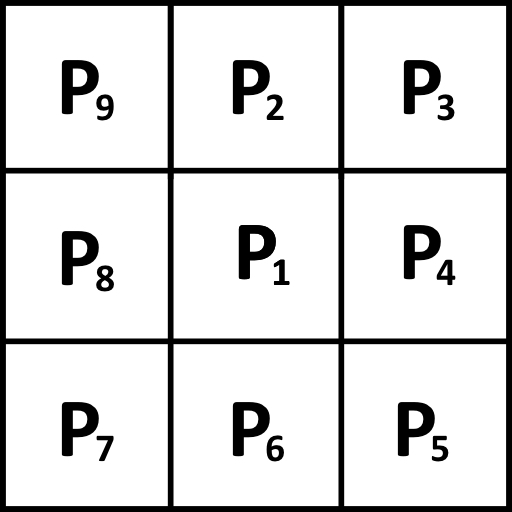
\includegraphics[width=4cm]{images/kernel.jpg}
    \caption{Strukturni element}
    \label{fig:points_kernel}
\end{figure}

Kako bi se trenutna crna točka nad kojom se nalazi strukturni element klasificirala kao krajnja točka nužno je zadovoljiti sljedeći uvjet:$$\sum_{i=2}^{9} P_i = 1.$$
Za klasifikaciju točke kao točke presjecišta nužno je zadovoljiti sljedeći jedan od sljedeća dva uvjeta:$$P_2 + P_4 + P_6 + P_8 \geq 2$$ ili $$P_3 + P_5 + P_7 + P_9 \geq 2.$$

Kako broj krajnjih točaka i točaka presjecišta može biti više, a neuronska mreža na svoje ulaze prima vrijednosti iz intervala od nula do jedan, u vektoru značajki se koristi njihova recipročna vrijednost, ili nula ukoliko navedenih točaka nema.

\section{Statističke značajke}

Od statističkih značajki korištene su horizontalna, vertikalna i dijagonala projekcija. Kao početna pozicija slike se gleda gornji lijevi ugao i ima koordinate $(1, 1)$.

\subsection{Horizontalna i vertikalna projekcije}

Za sliku, horizontalna projekcija je definirana nad svakim retkom kao skup od tri elementa:
\begin{enumerate}
    \item broj crnih slikovnih elemenata u pojedinom retku,
    \item pozicija prvog crnog slikovnog elementa s lijeva i
    \item pozicija prvog crnog slikovnog elementa s desna.
\end{enumerate}
Kako bi navedeni elementi bili neovisni o dimenziji slike, pojedini element se dijeli sa širinom slike, što uostalom postavlja dobivene brojeve u interval od nula do jedan, što zapravo savršeno odgovara kao ulaz neuronskoj mreži.

Što se tiče vertikalne projekcije, ona je definirana nad svakim stupcem slike kao skup od tri elementa:
\begin{enumerate}
    \item broj crnih slikovnih elemenata u pojedinom retku,
    \item pozicija prvog crnog slikovnog elementa od vrha i
    \item pozicija prvog crnog slikovnog elementa od dna.
\end{enumerate}
Iz istih razloga kao i kod horizontalne projekcije, pojedini element se dijeli sa visinom slike.

Na primjeru slike \ref{fig:hv_projection} za treći redak horizontalna projekcija bi bila $(0.5, 0.5, 0.83)$. Vertikalna projekcija za treći stupac bi bila $(0.16, 0.5, 0.5).$

\begin{figure}[htb]
    \centering
    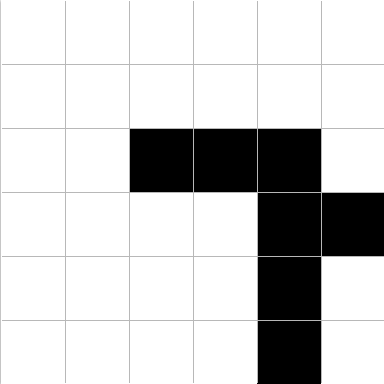
\includegraphics[width=5cm]{images/hvProj.png}
    \caption{Primjer za horizontalnu i vertikalnu projekciju}
    \label{fig:hv_projection}
\end{figure}

\subsection{Dijagonalna projekcija}

Dijagonalna projekcija je relativno nova tehnika izlučivanja značajki, koju su predstavili Pradeep, Srinivasan i Himavathi u svom radu 2011. godine  \citep{diagonal2011}.

Ulazna slika je dimenzija $30 \times 30$ točaka. Slika se zatim podjeli na 36 jednakih zona dimenzija $5 \times 5$. Svaka zona ima devet dijagonala i kretanjem po svakoj od dijagonala računa se koeficijent dijagonale tako da se broj točaka objekta, odnosno crnih točaka, dijeli s ukupnim brojem elemenata u toj dijagonali. Nakon što se prođu sve dijagonale u zoni, koeficijenti dijagonala se zbroje i podjele s ukupnim brojem dijagonala u zoni i na taj način se dobiva koeficijent pojedine zone. Primjer obilaska dijagonala dan je na slici \ref{fig:diagonals}.
\begin{figure}[htb]
    \centering
    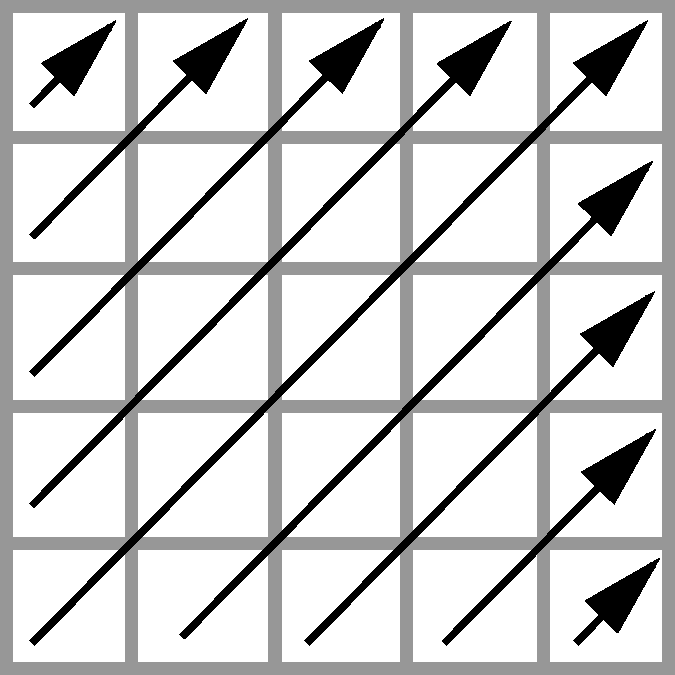
\includegraphics[width=5cm]{images/diagonal_arrows.pdf}
    \caption{Smjer obilaska dijagonala u zoni}
    \label{fig:diagonals}
\end{figure}

Uz navedenih 36 značajki, još se pridodaje 12 značajki koje računaju prosječni koeficijent zona za pojedini redak i pojedini stupac što ukupno daje 48 značajki za sliku dimenzija $30 \times 30$. Implementacija algoritma za izračunavanje koeficijenta pojedine zone u programskom jeziku \emph{Java} dana je sljedećim izvornim kodom.
\lstset{language=Java, tabsize=2}
\begin{lstlisting}
private double calculateZone(int[][] zone) {
    int count = 2 * ZONE_SIZE - 1;
    double sum = 0;
    for (int i = 0; i < count; i++) {
        int z = i < ZONE_SIZE ? 0 : i - ZONE_SIZE + 1;
        int sliceSize = i - z + 1;
        int sliceSum = 0;
        for (int j = z; j < sliceSize; j++)
            if (zone[j][i - j] == 1) sliceSum++;
        sum += sliceSum / (double) sliceSize;
    }
    return sum / count;
}
\end{lstlisting}
